\documentclass[a4paper]{article}

\usepackage[utf8]{inputenc}
\usepackage[portuguese]{babel}
\usepackage{a4wide}
\usepackage[pdftex]{hyperref}
\usepackage{graphicx}
\usepackage{wrapfig}
\usepackage{amsmath}
\usepackage{verbatim}
\usepackage{caption}
\usepackage{subcaption}
\usepackage{float}
\usepackage{blochsphere}



\begin{document}

\begin{titlepage}
\begin{center}



\includegraphics[width=0.4\textwidth]{logo.jpg}\\[0.5cm]

\vspace{10mm}

{\huge Universidade do Minho - Escola de Engenharia}\\[0.5cm]

{\large Relatório do trabalho prático de Computação Gráfica}\\[0.5cm]

\vspace{10mm} 

% Title
\rule{\linewidth}{0.5mm} \\[0.4cm]
{ \huge \bfseries Fase 1 – Primitivas Gráficas \\[0.4cm] }
\rule{\linewidth}{0.5mm} \\[1.5cm]

% Author and supervisor
\noindent
\begin{minipage}{0.4\textwidth}
  \begin{flushleft} \large
    \emph{Autores :}\\
    Daniel Maia \textsc{(A77531)}\\
    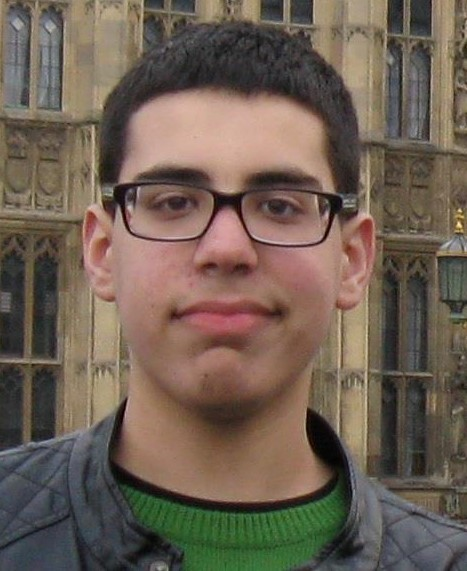
\includegraphics[width=1.5cm]{./imagens/daniel.jpg}\break
    Diogo Silva\textsc{(A78034)}\\
    
\includegraphics[width=1.5cm]{./imagens/afonso.jpg}\break
    Marco Silva\textsc{(A79607)}\\
    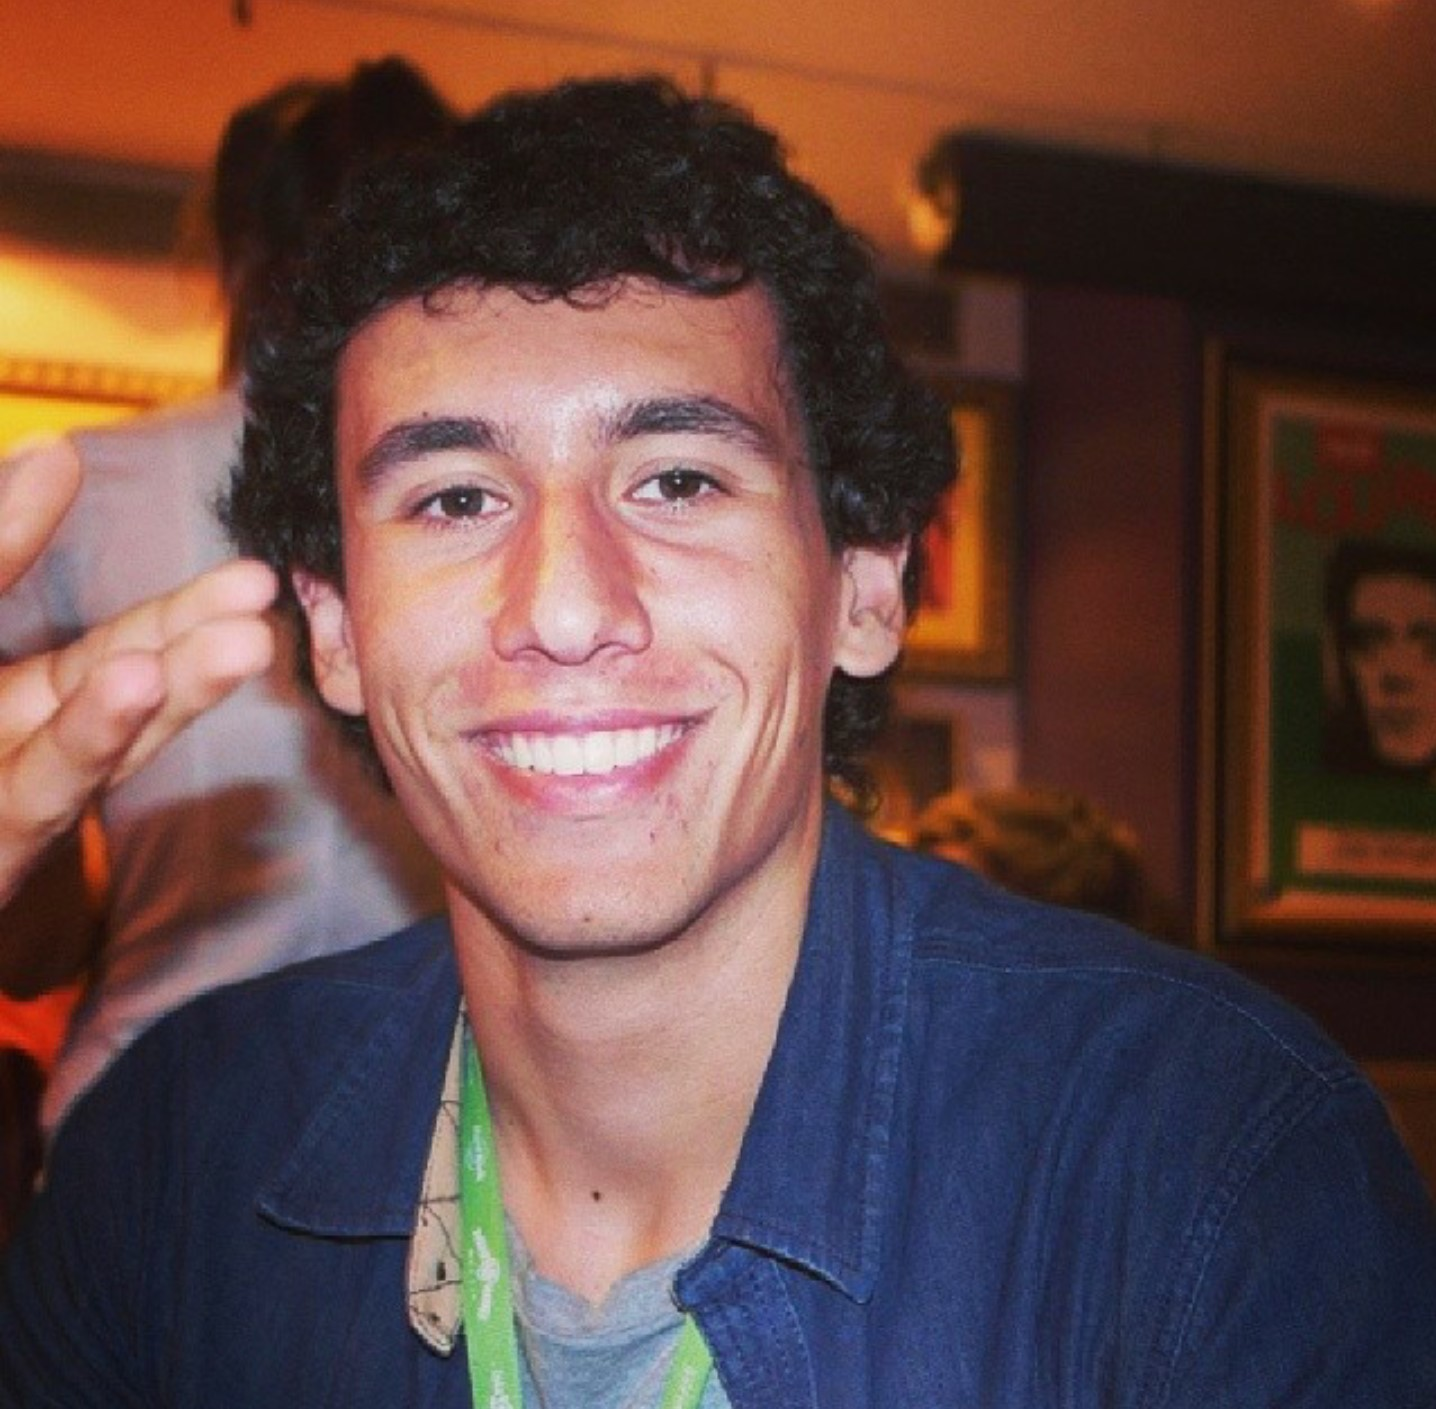
\includegraphics[width=1.5cm]{./imagens/marco.jpg}\break
  \end{flushleft}
\end{minipage}%
\vfill

% Bottom of the page
{\large Versão 1.0 \\ \today}

\end{center}
\end{titlepage}


\begin{abstract}

\hspace{3mm} O objetivo desta fase do trabalho envolve desenvolver duas aplicações. Uma, designada de \emph{Generator}, será responsável por gerar ficheiros com a informação relativa a um modelo, especificamente, os seus vértices. Para tal, receberá um conjunto de parâmetros necessários para a criação do modelo através da linha de comandos, incluindo o tipo de figura a ser gerada e as suas dimensões, bem como o nome e localização do ficheiro onde a informação será guardada. A outra aplicação, batizada de \emph{Engine}, terá a responsabilidade de ler de um ficheiro de configuração, escrito em XML, e, a partir deste, demonstrar os modelos anteriormente gerados.

\par Para esta fase, foi definido um conjunto de figuras que o \emph{Generator} suportará:

\begin{itemize}
    \item Plano (\emph{Plane}), representado por um quadrado centrado na origem, constituído por dois triângulos;
    \item Cubo (\emph{Box}), centrado na origem, cujas faces podem ser divididas em partes menores pelo utilizador no momento de geração;
    \item Esfera (\emph{Sphere}), centrado na origem, com um determinado raio e número de divisões horizontais e verticais;
    \item Cone, centrado na origem, com um determinado raio, altura e número de divisões horizontais e verticais.
\end{itemize}

\end{abstract}

\pagebreak
\tableofcontents

\pagebreak

% ===================================================
\section{Introdução}

\hspace{8mm} O objetivo deste projeto é desenvolver uma cena gráfica baseada num
motor 3D. Para tal são necessárias duas componentes: o \textit{generator} e o
\textit{engine}.

\hspace{3mm} Primeiramente, é executado o \textit{generator}. Este é responsável por
produzir todos os pontos necessários para a construção de uma
determinada primitiva gráfica. Após o cálculo dos pontos, estes são
guardados num ficheiro com a extensão \textbf{3d}.

\hspace{3mm} De seguida, a execução é encadeada com o componente \textit{engine}. Este analisa um ficheiro XML e com base na informação presente no mesmo, recorre aos ficheiros \textbf{3d} para carregar os pontos, que são consequentemente usados para desenhar as primitivas gráficas.

\hspace{3mm} Por último, para a realização do projeto foi utilizado o OpenGL Utility Toolkit (GLUT), que possibilita a escrita de programas em OpenGL independentemente do sistema de janelas. Adicionalmente, foi usada a linguagem C++ para a escrita do código e o \textit{pugixml} como biblioteca de processamente de XML.


% ===================================================
\section{Descrição do Trabalho e Análise de Resultados}

\subsection{Generator}

\hspace{8mm} Antes de abordar qualquer pormenor mais técnico relacionado com a geração dos pontos para as diversas figuras a desenhar, é importante explicitar que foi definida uma norma para a escrita nos ficheiros que irão representar as figuras abaixo descritas. Desta forma, foi estabelecido que em cada uma das linhas estarão presentes as 3 coordenadas em formato cartesiano com a ordem x, y e z, separadas por espaços, ficando assim em cada linha toda a informação necessária para a representação de um ponto.

\subsubsection{Plano} % nº de triângulos = 2

\hspace{8mm} No contexto do trabalho, o plano trata-se de um quadrado com um comprimento N passado por argumento na linha de comandos. Como tal, é necessário apenas determinar quatro pontos com os quais se poderá definir os dois triângulos que o constituirão. O plano está centrado em \emph{xz}, logo, os pontos seguem o formato (\emph{x, 0, z}), x e z sendo $\pm$ \( \frac{N}{2} \). Para manter a semântica do \emph{OpenGL}, dois destes pontos terão um duplicado no ficheiro que guardará a figura.

\begin{figure}[h!]
\centering
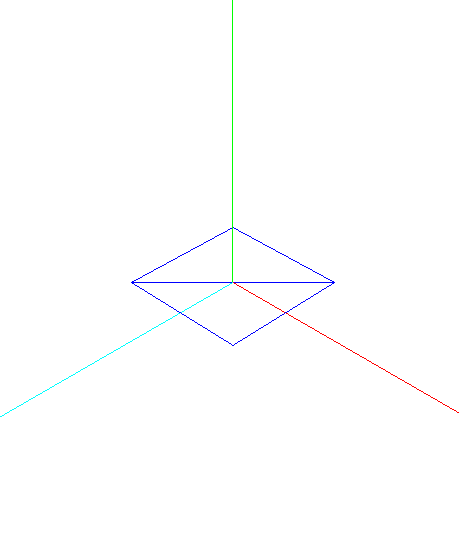
\includegraphics[width=5cm]{./imagens/plane.png}
\caption{Representação gráfica de um plano.}
\label{fig:plane}
\end{figure}

\subsubsection{Box} % nº de triângulos = 6 * (2^divisions)

\hspace{8mm} A primitiva gráfica \textit{box} tem como características o comprimento (z), a largura (x), a altura (y) e opcionalmente o número de divisões de cada face.

\begin{figure}[h!]
\centering
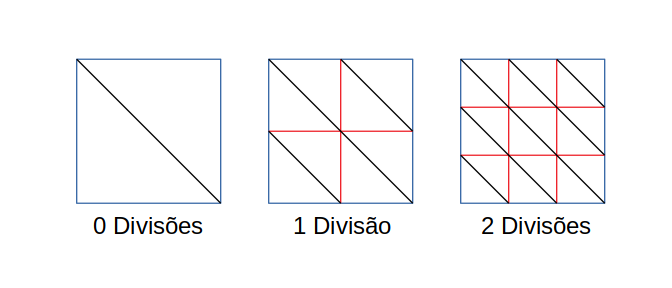
\includegraphics[width=12cm]{./imagens/divisions.png}
\caption{Aplicação do conceito de divisões.}
\label{fig:divisions}
\end{figure}

\hspace{3mm} Dado que as dimensões da \textit{box}, isto é, o \textbf{x}, \textbf{y} e \textbf{z} caracterizam o comprimento de cada um dos lados foi necessário dividir cada uma das medidas por dois. Desta forma, o centro da \textit{box} fica centrado na origem do referencial.

\hspace{3mm} De seguida, partiu-se para a conceção de como seriam implementadas as divisões. Primeiramente, tentou-se perceber qual a relação entre o incremento, ou seja, a base do triângulo, o número de divisões e o comprimento do lado. No final surgiu a seguinte fórmula:

\[ incremento_x = x / num\_divisions \]

\hspace{3mm} Deste modo, o próximo passo seria arranjar um algoritmo para desenhar os triângulos numa determinada face, respeitando o número de divisões. Assim sendo, decidiu-se que o ponto (\textit{master point} - MP) pelo qual nos guiaríamos seria, em toda e qualquer situação, o canto inferior esquerdo. Efetivamente, começaríamos a construir a face no quanto inferior esquerdo e os próprios triângulos teriam como ponto de referência o seu próprio canto inferior esquerdo.

\hspace{3mm} A título exemplificativo, realizamos um protótipo do que seria realizar a face frontal com 5 divisões. [\ref{fig:face5}]

\begin{figure}[h!]
\centering
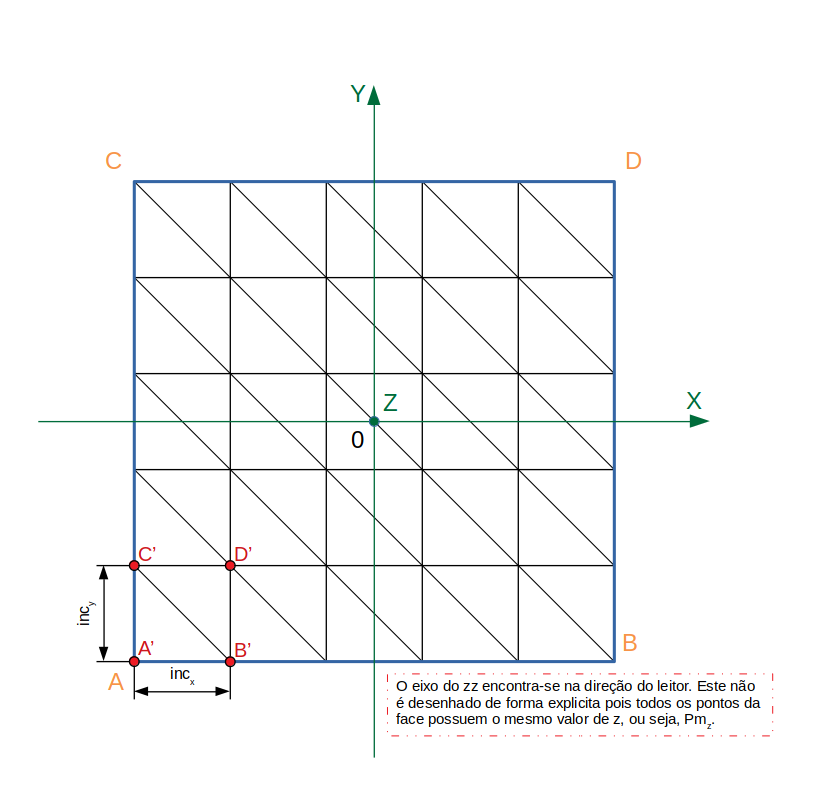
\includegraphics[width=13cm]{./imagens/face.png}
\caption{Face frontal com 5 divisões.}
\label{fig:face5}
\end{figure}

\hspace{3mm} De facto, seguindo a regra do MP começa-se a desenhar sempre do canto inferior esquerdo. De seguida, desenha-se a linha e no final desta, sobe-se para o início da linha seguinte e repete-se o processo até toda a face estar concluída. Para tal, é preciso conhecer os valores que se encontram na figura \ref{fig:face5}.

\[ MP (-(x/2), -(y/2), z/2) \]

\[ inc_x = x / divisions \]

\[ inc_y = y / divisions \]

\[ A'(MP_x, MP_y, MP_z) \]

\[ B'(MP_x + inc_x, MP_y, MP_z) \]

\[ C'(MP_x, MP_y + inc_y, MP_z) \]

\[ D'(MP_x + inc_x, MP_y + inc_y, MP_z) \]

\hspace{3mm} De forma, a  desenhar os primeiros dois triângulos deve-se inserir os pontos, na seguinte ordem, A', B', C' para o primeiro triângulo e C', B' e D' para o triângulo invertido. Após o desenho do primeiro quadrado (triângulo normal + triângulo invertido) é necessário atualizar o MP apenas numa das variáveis. Esta variável varia conforme a face que esteja a ser desenhada, contudo no exemplo em questão é o \textbf{x}.

\[ MP_x = MP_x + inc_x \]

\hspace{3mm} Contudo, chegando à última coluna é necessário subir para a linha seguinte. Neste caso, não basta atualizar uma das variáveis mas sim duas. No exemplo acima, são o \textbf{x} e o \textbf{y} que sofrem mudanças. O \(MP_x\) volta à coordenada original e o \(MP_y\) é simplesmente incrementado.

\[ MP_x = -(x/2) \]

\[ MP_y = MP_y + inc_y \]

\hspace{3mm} Finalmente, basta correr o algoritmo para cada uma das faces. Como resultado teremos uma \textit{box} com as dimensões x, y, z e com n divisões.



\subsubsection{Cone} % nº de triângulos = ( 2 * (stacks * slices) ) + slices ; pontos repetem 6 vezes

\hspace{8mm} Para desenhar o cone de um modo mais detalhado, este será separado num número de cortes horizontais (\emph{stacks}) e verticais (\emph{slices}), permitindo-nos observar a sua face curva como um conjunto de retângulos, que por sua vez, serão divididos num par de triângulos, e observar a sua base como um conjunto de triângulos que partilham um vértice posicionado no centro da mesma.  Deste modo, será possível desenhar o cone de modo a que tenha a aparência de ser realmente curvo, apesar de ser, na verdade, um conjunto de triângulos. Permitirá também colorir o cone de modo a dar uma ilusão de existir uma fonte de luz ao espetador.

\hspace{3mm} Para facilitar o futuro uso de funções de transformação geométrica, decidiu-se desenhar o cone coincidindo o seu centro e alinhando o seu vértice com o eixo \emph{yy}. Deste modo, sabe-se que o vértice estará posicionado no ponto (\emph{0, \( \frac{h}{2} \), 0}) e os pontos da base estarão posicionados em (\emph{x, \( -\frac{h}{2} \), z}) a uma distância \emph{r} do eixo \emph{yy}, sendo \emph{h} a altura do cone, definida pelo utilizador. Portanto, é necessário assegurar que \emph{r} seja constante. No entanto, fazê-lo através de coordenadas cartesianas prova ser extremamente complicado, portanto, utilizou-se coordenadas polares, recorrendo aos fundamentos da matemática. Sabendo que \emph{y} se mantém constante, pode-se considerar momentaneamente que se depara com um plano alinhado a \emph{xz}. No sistema de coordenadas cartesiano, $r = \sqrt{(x2 - x1)^2 + (z2 - z1)^2}$. A partir daqui, é possível definir três pontos não colineares, (x1,z1), (x2,z1) e (x2,z2), com os quais se pode definir um ângulo $\alpha$. Recorrendo ao processo inverso, para um dado ângulo $\alpha$, é possível determinar \emph{x} e \emph{z} através do Teorema Fundamental da Trigonometria: $\sqrt{sin^2(\alpha) + cos^2(\alpha)} = 1$. Aplicando o Teorema a \emph{r}, $\sqrt{(r*sin(\alpha))^2 + (r*cos(\alpha))^2} = r$. Por convenção, define-se $x = r*sin(\alpha)$ e $z = r*cos(\alpha)$. No contexto do OpenGL, determina-se $\alpha$ através da fórmula $\alpha = i * \frac{2\pi}{slices}, 0 \leq i < slices$.

\begin{figure}[h!]
\centering
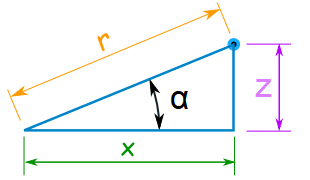
\includegraphics[width=7cm]{./imagens/coordinates-triangle.png}
\caption{.}
\label{fig:cp_triangle}
\end{figure}

\hspace{3mm} Expandir este conceito ao espaço requer considerar um segundo ângulo $\beta$. No entanto, no caso do cone prescinde-se deste graças ao facto de que se sabe que todos os pontos se encontrarão num ponto (\emph{x}, $ -\frac{h}{2} + j * \frac{h}{stacks}$, z), distando $r - j * \frac{r}{stacks}$ do eixo \emph{yy}, $0 \leq \emph{j} \leq \emph{stacks}$. 

\hspace{3mm} Deste modo, tem-se um método de determinar todos os pontos que serão introduzidos no ficheiro que guardará a figura. Para cada valor de \emph{i} e \emph{j}, calcular-se-á um ponto, de coordenadas ($(r - j \frac{r}{stacks}) * sin(i * \frac{2\pi}{slices}), -\frac{h}{2} + j * \frac{h}{stacks}, (r - j \frac{r}{stacks}) * cos(i * \frac{2\pi}{slices})), 0 \leq i < slices, 0 \leq j \leq stacks$. É necessário então aplicar o método num formato legível para o OpenGL. Isto obriga, no entanto, que cada ponto seja repetido no ficheiro seis vezes, resultando num ficheiro de tamanho maior, mas lido de um modo mais rápido pelo OpenGL.

\pagebreak

\begin{figure}[h!]
\centering
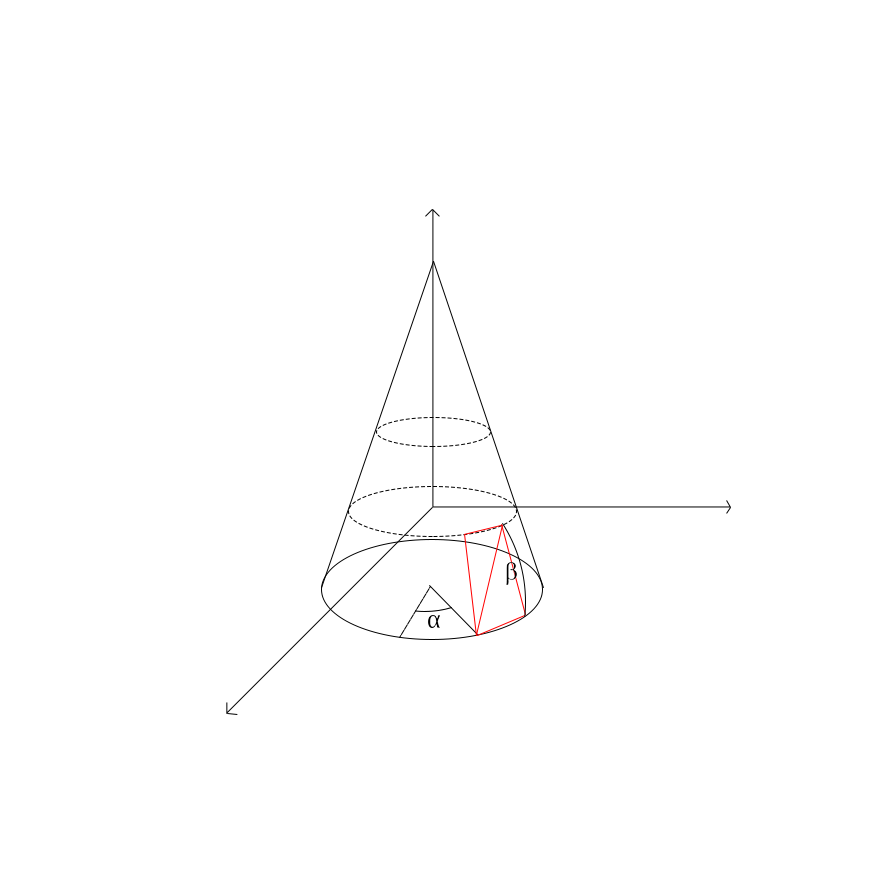
\includegraphics[width=7cm]{./imagens/cone.png}
\caption{Representação de um cone utilizando coordenadas polares.}
\label{fig:cone}
\end{figure}

\subsubsection{Esfera} % nº de triângulos = 2 * stack * slices

\hspace{8mm} Para a construção da esfera, inicialmente foram estudadas as várias possibilidades para a representação das coordenadas. O mais comum seria a utilização de coordenadas cartesianas mas, uma vez que para o desenho da esfera pretendemos representar superfícies planas foram utilizadas coordenadas polares, sendo mais adequadas ao problema.

\begin{figure}[h!]
\centering
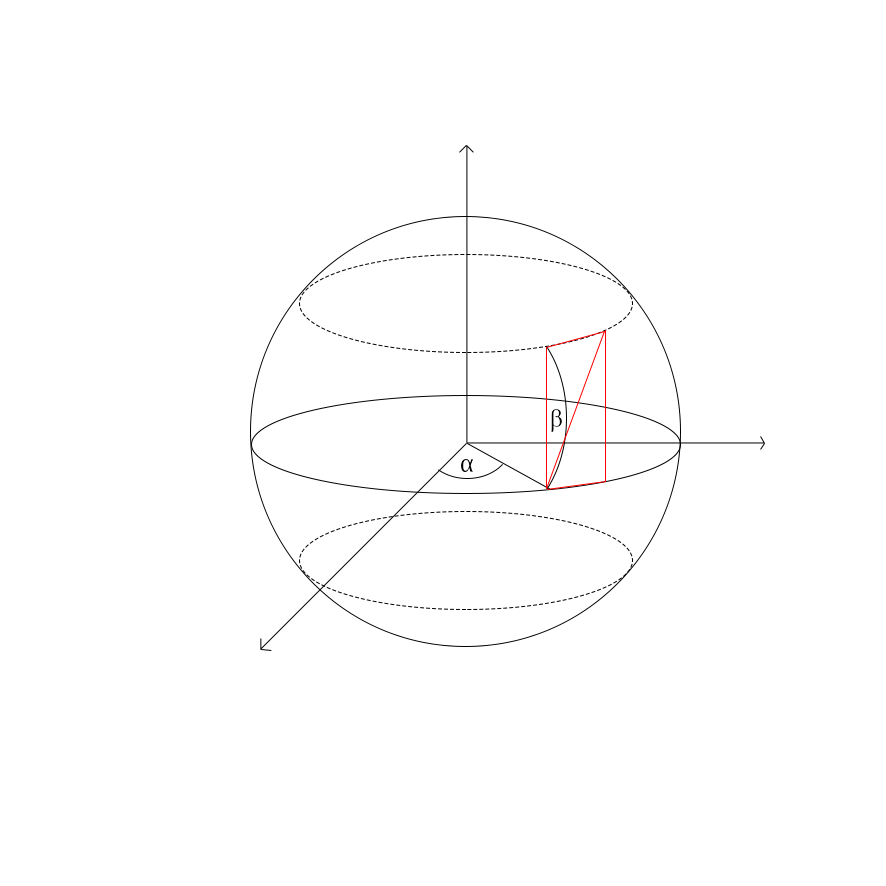
\includegraphics[width=7cm]{./imagens/sphere.png}
\caption{Representação da esfera utilizando coordenadas polares e demonstração do passo iterativo de desenho de triângulos.}
\label{fig:sphere}
\end{figure}

\hspace{3mm} Uma vez que, juntamente com a especificação do raio da esfera a desenhar, é também fornecido o número de \emph{slices} (divisões verticais) e \emph{stacks} (divisões horizontais), conclui-se que as variações dos ângulos $\alpha$ e $\beta$ que se podem ver representados na figura acima, irão estar diretamente relacionadas com o número de \emph{slices} e \emph{stacks} respetivamente.

\hspace{3mm} Primeiramente, são calculados os incrementos quer em $\alpha$ quer em $\beta$ com base no valor de \emph{slices} e \emph{stacks} que são necessários. No caso das \emph{slices} (correspondente ao $\alpha$ na figura), $increment1 = (2\Pi) / \emph{slices}$ uma vez que terão de ser desenhadas \emph{slices} em redor de toda a esfera enquanto que para as \emph{stacks}, $increment2 = \Pi / \emph{stacks}$. Para as \emph{stacks}, apenas é necessário percorrer $\Pi$ radianos visto que o desenho das \emph{slices} já percorrem $2\Pi$ radianos cobrindo assim por completo a superfície da esfera.

\hspace{3mm} Tendo este raciocínio consolidado, apenas é necessário explicitar os passos a tomar em cada uma das iterações. Tendo em atenção a imagem acima apresentada, podemos ver o desenho a vermelho de dois triângulos que juntos representam um retângulo. As coordenadas destes pontos são determinadas com base nos ângulos atuais quer de $\alpha$ e $\beta$ adicionando os incrementos respetivos calculados anteriormente.
\par Este raciocínio encontra-se dentro de dois ciclos, cada um com o número de \emph{stacks} e \emph{slices} indicados.


\subsection{Engine}

\subsubsection{Formato XML}

\hspace{8mm} O formato XML surge neste projeto como "guião" da cena a ser desenhada uma vez que tem nele descrito os ficheiros de pontos que devem ser desenhados e numa fase mais avançada, instruções como \emph{translate} ou \emph{rotate}.

\hspace{3mm} Nesta primeira fase, o ficheiro XML é bastante simples, sendo apenas constituído por uma \emph{tag} scene que por sua vez alberga a \emph{tag} model com o atributo \emph{file} que representa o nome do ficheiro de pontos a desenhar.

\hspace{3mm} Tendo assim bem definida a estruturação do ficheiro, apenas é necessário aceder aos conteúdos deste ficheiro e extrair a informação necessária, neste caso são apenas necessários os nomes dos ficheiros de pontos.

\subsubsection{Leitura e Desenho}

\hspace{8mm} Uma vez extraída a informação necessária do ficheiro XML,utilizando a biblioteca \href{https://github.com/zeux/pugixml}{pugixml} \cite{pugixml}, pode-se proceder ao tratamento dos ficheiros em causa. Primeiramente, estes são abertos apenas com permissões de escrita e é feita a leitura linha a linha dos mesmos.

\hspace{3mm} Assim sendo, dando ênfase à estrutura definida anteriormente dos ficheiros \textbf{3d}, foi utilizada uma função \emph{split} que dada uma string, um delimitador e um vetor, procede à divisão da mesma colocando o resultado no vetor indicado.
Tendo a informação já devidamente tratada, basta proceder à conversão do formato \emph{string} para \emph{float} recorrendo à função \emph{atof}. Assim, percorrendo todas as linhas do ficheiro e fornecendo os dados extraídos ao OpenGL, as figuras são construídas na sua totalidade.

\newpage
% ===================================================
\section{Conclusões e Sugestões}

\hspace{8mm} Após experimentação, concluiu-se que a geração de ficheiros com alguma redundância, mas que podem ser lidos sequencialmente pelo \textit{engine}, habilitam uma melhor performance num todo, quando comparados com ficheiros gerados com o intuito de serem mais eficientes em termos de armazenamento, o que consequentemente requereria uma maior computação no componente \textit{engine} aquando da construção das primitivas gráficas, além de provocar uma pior legibilidade do código.

\hspace{3mm} O projeto utiliza o \textit{generator} para gerar os pontos que formam as primitivas gráficas e, consequentemente, executa o \textit{engine} que transformará os pontos em objetos concretos, numa cena. Efetivamente, esta dualidade permite que o componente \textit{engine} seja completamente independente da primitiva que se encontre a desenhar. Deste modo, este pode ser usado para desenhar qualquer figura, quer esta seja mais ou menos complexa, incluindo primitivas não suportadas pelo \textit{generator}.

\hspace{3mm} A modularidade com que o motor 3D foi concebido permitirá que, no futuro, facilmente se acrescente primitivas gráficas e funcionalidades mais exigentes a nível computacional.

\newpage
% =========================================================
\bibliographystyle{unsrt}
\bibliography{biblio}


\end{document}
